\documentclass[12pt,a4paper]{article}
\usepackage[T1]{fontenc}
\usepackage{amsmath}
\usepackage{amssymb}
\usepackage{graphicx}
\usepackage[UTF8,heading=true]{ctex}
\usepackage{geometry}
\usepackage{diagbox}
\usepackage[]{float}
\usepackage{xeCJK}
\usepackage{indentfirst}
\usepackage{multirow}
\usepackage[section]{placeins}
\usepackage{caption}
\usepackage{listings}
\usepackage{xcolor}

% 设置代码块样式
\lstset{
  frame=tb,
  aboveskip=3mm,
  belowskip=3mm,
  showstringspaces=false,
  columns=flexible,
  framerule=1pt,
  rulecolor=\color{gray!35},
  backgroundcolor=\color{gray!5},
  basicstyle={\small\ttfamily},
  numbers=none,
  numberstyle=\tiny\color{gray},
  keywordstyle=\color{blue},
  commentstyle=\color{green!50!black},
  stringstyle=\color{mauve},
  breaklines=true,
  breakatwhitespace=true,
  tabsize=3,
}

\setCJKfamilyfont{zhsong}[AutoFakeBold = {5.6}]{STSong}
\newcommand*{\song}{\CJKfamily{zhsong}}

\geometry{a4paper,left=2cm,right=2cm,top=0.75cm,bottom=2.54cm}

\newcommand{\experiName}{prj4}%实验名称
\newcommand{\name}{28}
\newcommand{\student}{刘景平、张钰堃、付博宇}%姓名
\newcommand{\others}{$\square$}
\newcommand{\sectionfont}{\song\textbf}

\ctexset{
    section={
        format+=\raggedright
    },
    subsection={
        name={\quad,.}
    },
    subsubsection={
        name={\qquad,.}
    }
}

\begin{document}
\noindent

\begin{center}

    \textbf{\song \zihao{-2} \ziju{0.5} 计算机体系结构(研讨课)实验报告}
    
\end{center}


\begin{center}
    \kaishu \zihao{5}
    \noindent \emph{实验项目}\underline{\makebox[5em][c]{\experiName}}
    \emph{小组编号}\underline{\makebox[5em][c]{\name}} 
    \emph{组员姓名}\underline{\makebox[20em][c]{\student}}
    {\noindent}
    \rule[5pt]{17.7cm}{0.2em}

\end{center}


\section{\sectionfont 逻辑电路结构与仿真波形的截图及说明}
    \subsection{exp12}
        \subsubsection{增加CSR模块}
            1.需要为CSR模块单独写一个verilog文件,作为专用于CSR的寄存器堆,按照教材上的指导加入一系列输入输出信号,
            并在头文件中加入每个CSR的寄存器号,每个CSR各部分的位置等信息:
            \begin{figure}[H]
                \centering
                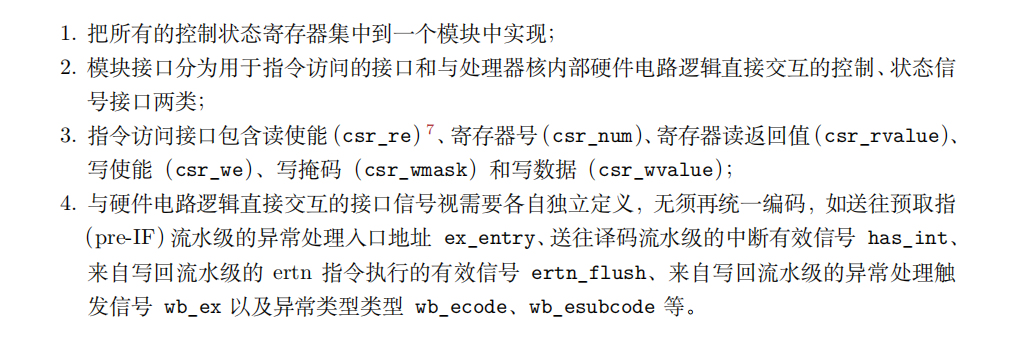
\includegraphics[width=0.8\textwidth]{创建CSR-1.png}
                \caption{讲义上关于创建CSR模块的指导}
            \end{figure}

            \begin{figure}[H]
                \centering
                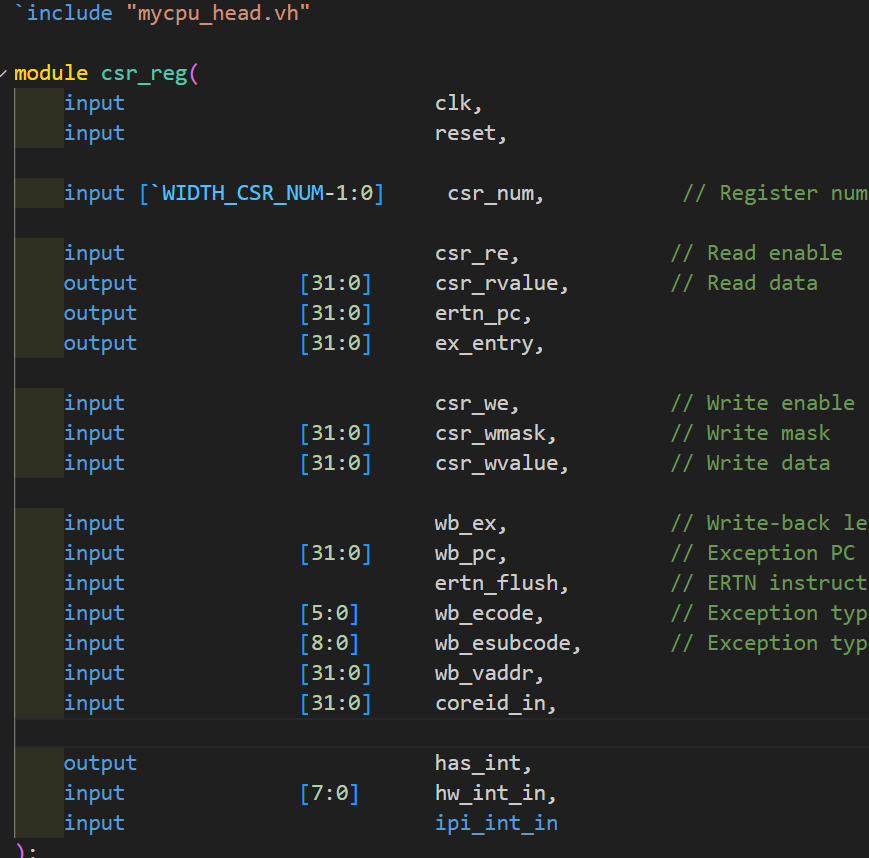
\includegraphics[width=0.8\textwidth,height=0.4\textheight]{修改头文件.png}
                \caption{创建CSR模块}
            \end{figure}

            \begin{figure}[H]
                \centering
                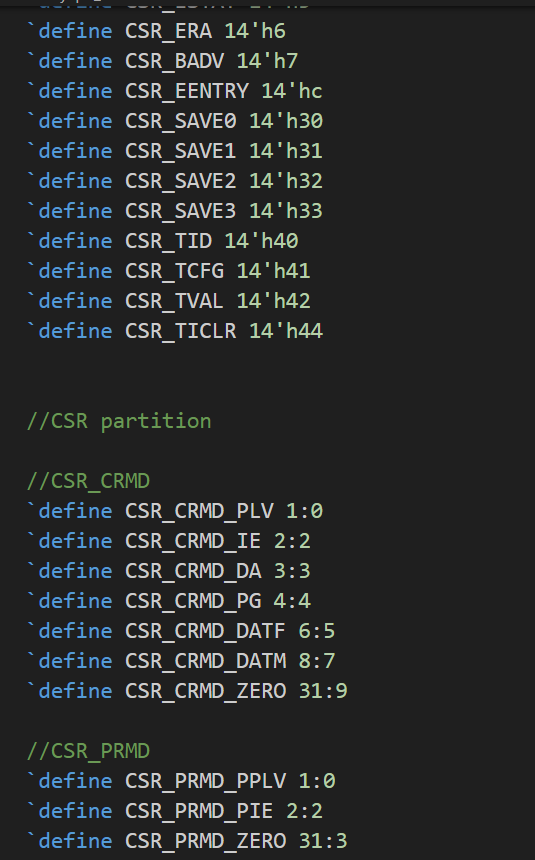
\includegraphics[width=0.8\textwidth,height=0.5\textheight]{创建CSR-2.png}
                \caption{修改头文件}
            \end{figure}
            \par
            2.根据讲义上的例子添加CRMD、PRMD、ESTAT、ERA、EENTRY、SAVE0~3八个控制状态寄存器。并按照指令集手册的要求添加关于read value的设置
            \begin{figure}[H]
                \centering
                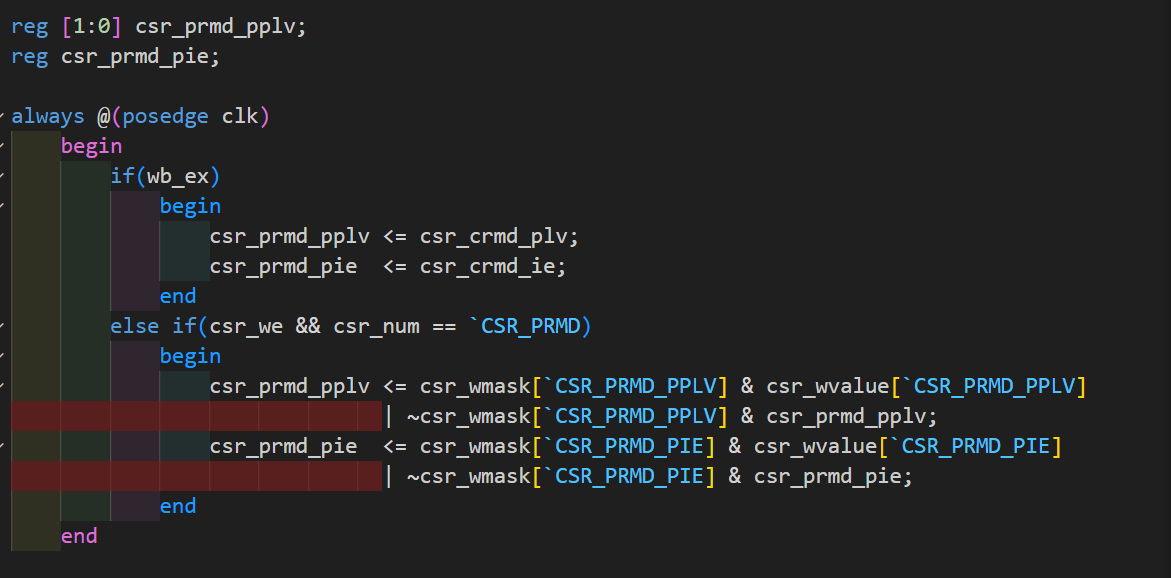
\includegraphics[width=0.8\textwidth]{PRMD.png}
                \caption{PRMD寄存器的设置}
            \end{figure}

            \begin{figure}[H]
                \centering
                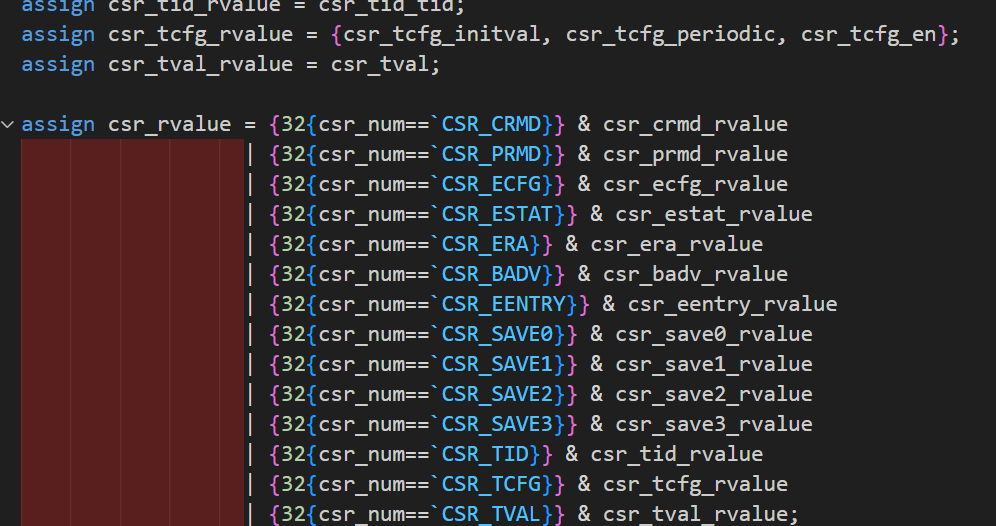
\includegraphics[width=0.8\textwidth]{rvalue.png}
                \caption{设置rvalue}
            \end{figure}
            \par
        
        \subsubsection{修改五个流水线模块}
            1.在IF中对nextpc进行修改,加入出现中断和例外,以及异常处理返回的情况
            \begin{lstlisting}[language=Verilog]
                wire [31:0] next_pc;    //nextpc from branch or sequence
                assign next_pc = (has_int || wb_ex)? ex_entry : ertn_flush? ertn_pc : br_taken? br_target : seq_pc;
            \end{lstlisting}
            \par
            2.在ID模块中加入对CSR读写指令有关的译码信号并增加和CSR有关的阻塞;
            \begin{lstlisting}[language=Verilog]
                wire csr_crush;
                assign csr_crush = (es_csr && (ex_crush1 || ex_crush2)) || (ms_csr && (mem_crush1 || mem_crush2)); 
            \end{lstlisting}

            \begin{figure}[H]
                \centering
                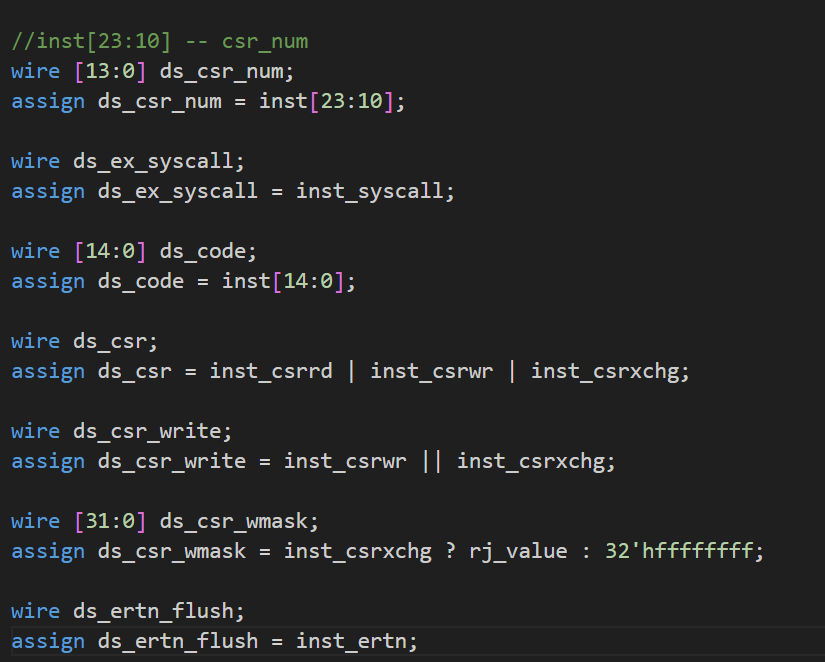
\includegraphics[width=0.8\textwidth,height=0.3\textheight]{csr读写译码.png}
                \caption{csr读写译码}
            \end{figure}
            \par
            3.在遇到ertn指令或者遇到中断和例外时,需要情况流水级间缓存:
            \begin{figure}[H]
                \centering
                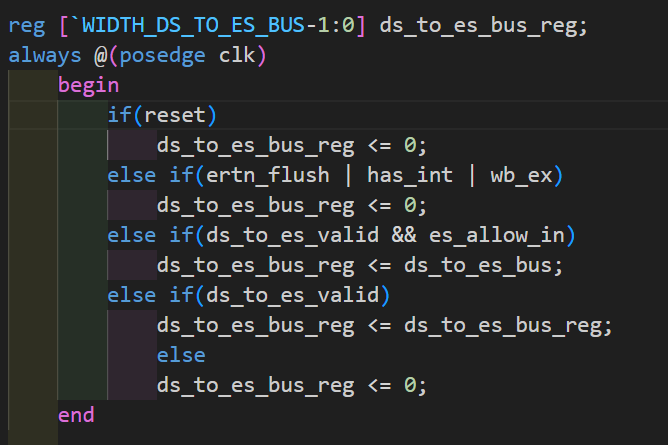
\includegraphics[width=0.8\textwidth]{清空流水级缓存.png}
                \caption{清空流水级间缓存}
            \end{figure}
            \par
            4.在最后一级WB级进行中断与异常的判断:
            \begin{figure}[H]
                \centering
                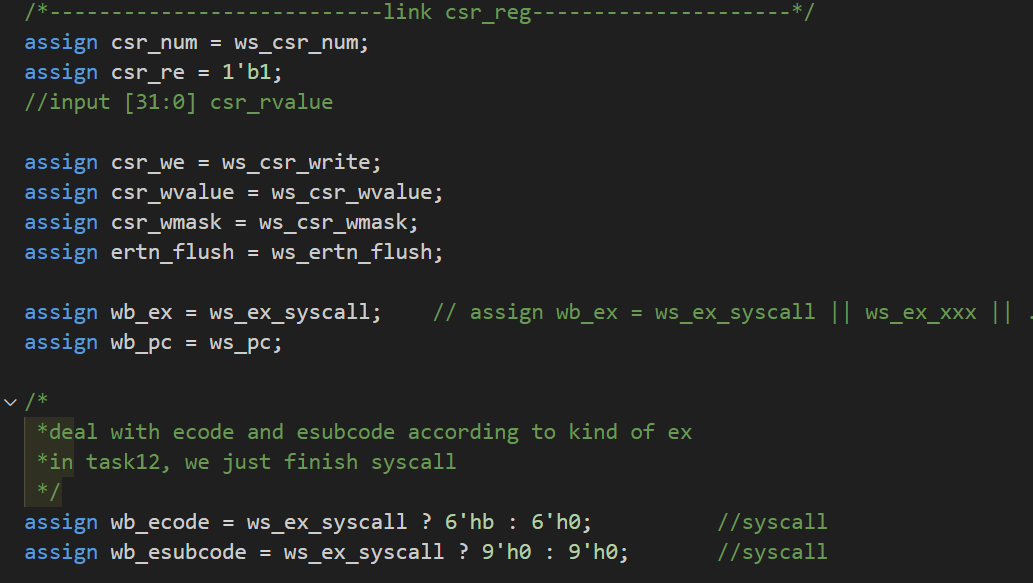
\includegraphics[width=0.8\textwidth]{在最后一级判断中断与异常.png}
                \caption{在最后一级判断中断与异常}
            \end{figure}
                
        
            
    \subsection{exp13}
        \subsubsection{添加转移指令}
          1.添加转移指令首先需要增加有关指令类型的译码信号,按照之前的格式,写明该指令的汇编代码和具体操作,以beq和bne指令为例:
          \par
          2.需要根据指令类型译码信号更改其他相关的译码信号,如gr-we、br-target等,剩余的指令通路与之前的转移指令相同。
          \par
          3.为了同时处理有符号数和无符号数的比较,需要利用加法进行判断,在ID模块中加入了一个小加法器。
          \begin{lstlisting}[language=Verilog]
            //imitation calcu slt and sltu in alu
          wire signed_rj_less_rkd;
          wire unsigned_rj_less_rkd;

          wire cin;
          assign cin = 1'b1;
          wire [31:0] adver_rkd_value;
          assign adver_rkd_value = ~rkd_value;
          wire [31:0] rj_rkd_adder_result;
          wire cout;
          assign {cout, rj_rkd_adder_result} = rj_value + adver_rkd_value + cin;

          assign signed_rj_less_rkd = (rj_value[31] & ~rkd_value[31])
                                        | ((rj_value[31] ~^ rkd_value[31]) & rj_rkd_adder_result[31]);
          assign unsigned_rj_less_rkd = ~cout;  
          \end{lstlisting}
          首先将rd中的值取反,然后将rj与~rd相加,并加入一个进位1,计算出一个33位的加法结果,其中最高位cout为进位。
          对于无符号数的比较而言,如果没有进位则说明rj小于rd,即unsigned\_rj\_less\_rkd为1。
          对于有符号数的比较而言,如果rj的符号为1,而rd的符号位为0,则可直接说明rj小于rd,即signed\_rj\_less\_rkd为1;
          如果rj和rd的符号位相同,则需要比较rj与~rd的加法结果的符号位,如果为1则说明rj小于rd,即signed\_rj\_less\_rkd为1。
        
        \subsubsection{添加st指令}
        在LoongArch指令集中st.b、st.h、st.w分别对应store byte(1字节)/halfword(2字节)/word(4字节),其中.h和.w分别要求地址2字节和4字节对齐。
        \par
        1.添加转移指令首先需要增加有关指令类型的译码信号,不再次举例
        \par
        2.st.b的四种偏移00、01、10、11分别对应mem-we为0001、0010、0100、1000。st.h的两种偏移00、10分别对应mem-we为0011、1100。如此对mem-we进行赋值。32位的wdata将8位数据重复4次,16位数据重复2次填满即可
        \par
        3.在EX中对未对齐的地址进行对齐操作,定义了一个写使能信号 w-strb 和真实写数据 real-wdata,根据 st-op 的不同情况进行选择
        \begin{lstlisting}[language=Verilog]
            wire [3:0] w_strb;  //depend on st_op
            assign w_strb =  es_st_op[0] ? 4'b1111 :
                             es_st_op[1] ? (es_unaligned_addr==2'b00 ? 4'b0001 : es_unaligned_addr==2'b01 ? 4'b0010 : 
                                            es_unaligned_addr==2'b10 ? 4'b0100 : 4'b1000) : 
                             es_st_op[2] ? (es_unaligned_addr[1] ? 4'b1100 : 4'b0011) : 4'b0000;
            wire [31:0] real_wdata;
            assign real_wdata = es_st_op[0] ? es_rkd_value :
                                es_st_op[1] ? {4{es_rkd_value[7:0]}} :
                                es_st_op[2] ? {2{es_rkd_value[15:0]}} : 32'b0;
        \end{lstlisting}\par
        4.对SRAM相关信号进行修改
        \begin{lstlisting}[language=Verilog]
            assign data_sram_en    = 1'b1;   
            assign data_sram_wen   = (es_mem_we && es_valid) ? w_strb : 4'b0000;
            assign data_sram_addr  = (es_mul_op != 0) ? {es_mul_result[31:2],2'b00} : {es_alu_result[31:2],2'b00};
            assign data_sram_wdata = real_wdata;   
        \end{lstlisting}

        \subsubsection{添加ld指令}
        
        \par
        1.添加转移指令首先需要增加有关指令类型的译码信号,与之前添加各项指令译码。
        \begin{lstlisting}[language=Verilog]
        assign inst_ld_b = op_31_26_d[6'h0a] & op_25_22_d[4'h0];
        assign inst_ld_h = op_31_26_d[6'h0a] & op_25_22_d[4'h1];
        assign inst_ld_bu = op_31_26_d[6'h0a] & op_25_22_d[4'h8];
        assign inst_ld_hu = op_31_26_d[6'h0a] & op_25_22_d[4'h9]; 
        \end{lstlisting}
        此外添加3位ld op,搭配res from mem信号标志当前执行的是哪个load指令,其中0位表示load byte,1位表示load half word,2位表示为有符号扩展。
        \begin{lstlisting}[language=Verilog]
        wire [2:0]  ld_op;
        assign ld_op[0] = inst_ld_b | inst_ld_bu;//load byte
        assign ld_op[1] = inst_ld_h | inst_ld_hu;//load half word
        assign ld_op[2] = inst_ld_h | inst_ld_b;//is signed 
        \end{lstlisting}
        大部分译码部分相关信号只用把原先只有ld.w信号的部分扩展成各类ld指令的信号,不再赘述。
        \par
        2.在EX级需要注意,由于载入的不再是按字节load,地址的后两位可能非零,这一数据需要传递到MEM级进行处理。此外,ld op也需要传递到MEM级来处理读取的数据。
        \begin{lstlisting}[language=Verilog]
        wire [1:0] es_unaligned_addr;
        assign es_unaligned_addr = (es_mul_op != 0) ? es_mul_result[1:0] : es_alu_result[1:0];
        assign es_to_ms_bus[72:71] = es_unaligned_addr;
        assign es_to_ms_bus[75:73] = es_ld_op; 
        \end{lstlisting}
        \par
        3.在MEM级根据ld op对读取的数据进行选择和扩充。
        \begin{lstlisting}[language=Verilog]
            wire [31:0] load_b_res,load_h_res;
            assign load_b_res   = (unaligned_addr == 2'h0) ? {{ms_ld_op[2]?{24{data_sram_rdata[7]}}:24'b0} ,data_sram_rdata[7:0]}
                    :(unaligned_addr == 2'h1) ? {{ms_ld_op[2]?{24{data_sram_rdata[15]}}:24'b0},data_sram_rdata[15:8]}
                    :(unaligned_addr == 2'h2) ? {{ms_ld_op[2]?{24{data_sram_rdata[23]}}:24'b0},data_sram_rdata[23:16]}
                    :(unaligned_addr == 2'h3) ? {{ms_ld_op[2]?{24{data_sram_rdata[31]}}:24'b0},data_sram_rdata[31:24]} : 32'b0;
            assign load_h_res   = (unaligned_addr[1]) ? {{ms_ld_op[2]?{16{data_sram_rdata[31]}}:16'b0} ,data_sram_rdata[31:16]}
                    :{{ms_ld_op[2]?{16{data_sram_rdata[15]}}:16'b0} ,data_sram_rdata[15:0]};
            assign mem_result   = ms_ld_op[0] ? load_b_res 
                    : ms_ld_op[1] ? load_h_res
                    : data_sram_rdata;
        \end{lstlisting}\par

\section{\sectionfont 实验过程中遇到的问题、对问题的思考过程及解决方法}
    \subsection{exp10}
        1.在添加乘法指令时,需要注意传递给乘法器的数据只可能是寄存器传来的数据,所以这里传给乘法器的数据为es rj value,es rkd value,而非cal src。
    \subsection{exp11}
        1.在添加有关ld.b,ld.h等指令有关扩展至32位的逻辑时,发现先判断后复制的逻辑会导致只有最后一位填充,而先扩充成24位在判断选择就能正常执行,具体指令如下:
        \begin{lstlisting}[language=Verilog]
            assign load_h_res   = (unaligned_addr[1]) ? {{24{ms_ld_op[2]?{data_sram_rdata[31]}:0}} ,data_sram_rdata[31:16]}
        :{{ms_ld_op[2]?{16{data_sram_rdata[15]}}:16'b0} ,data_sram_rdata[15:0]};
        // 0x8XXX -> 0x00018XXX
            
            assign load_h_res   = (unaligned_addr[1]) ? {{ms_ld_op[2]?{16{data_sram_rdata[31]}}:16'b0} ,data_sram_rdata[31:16]}
        :{{ms_ld_op[2]?{16{data_sram_rdata[15]}}:16'b0} ,data_sram_rdata[15:0]};
        // 0x8XXX -> 0xffff8XXX
        \end{lstlisting}
        猜测是由于前者会把扩展后的24位整体当作一位添加在原本的16位之前,然后自动填充15位0,导致实验结果与预期不同。修改成后者便能正常运行。
\section{\sectionfont 实验分工}
    张钰堃负责完成exp12,刘景平负责完成exp13。
\end{document}